%%%%%%%%%%%%%%%%%%%%%%%%%%%%%%%%%%%%%%%%%%%%%%%%%%%%%%%%%%%%%%%%%%%%%%%%%%%%%%%%%%
%%      Template using LaTeX  Tutorial tex files								%%
%%      																		%%
%%      Copyright Rho Vector Latex Tutorial 2021								%%
%%		rhovector <rhovector@gmail.com>			 								%%
%%		vivekadi <vivek.adishesha@gmail.com>,									%%
%%		chiranjitpatel <chiranjitpatel08@gmail.com>								%%
%%																				%%
%%																				%%	
%%      This program is FREE SOFTWARE; you can redistribute it and/or modify	%%
%%      it under the terms of the GNU General Public License as published by	%%
%%      the Free Software Foundation; either version 2 of the License, or		%%
%%      (at your option) any later version.										%%
%%      																		%%
%%      This program is distributed in the hope that it will be useful,			%%
%%      but WITHOUT ANY WARRANTY; without even the implied warranty of			%%
%%      MERCHANTABILITY or FITNESS FOR A PARTICULAR PURPOSE.					%%
%%      See GNU General Public License for more details.						%%
%%      																		%%
%%      You should have received a copy of the GNU General Public License		%%
%%      along with this program; if not, write to the Free Software				%%
%%      Foundation, Inc., 51 Franklin Street, Fifth Floor, Boston,				%%
%%      MA 02110-1301, USA.														%%
%%%%%%%%%%%%%%%%%%%%%%%%%%%%%%%%%%%%%%%%%%%%%%%%%%%%%%%%%%%%%%%%%%%%%%%%%%%%%%%%%%


\documentclass{article}

%% Used for multicol pages %%
\usepackage{multicol}

%% Used for images %%
\usepackage{graphicx}

%% USed for image location %%
\usepackage{float}

%% Used for subfigures and multiple image sets %%
\usepackage{caption}
\usepackage{subcaption}

\begin{document}
	
	
	%% Minipage is use to split the documant page in parts for independent editing and control %%
	%% ``minipage'' clock is invoked with perfectage of linewidth as the size of the minipages %%
	%% Here is an example to create distinguish between in a document with minipage %%
	\begin{minipage}{0.5\linewidth}
		\textbf{Advantges}		
		\begin{itemize}
			\item one
			\item two
			\item three
		\end{itemize}	
	\end{minipage}	
	\begin{minipage}{0.5\linewidth}
		\textbf{Disadvantges}	
		\begin{itemize}
			\item one
			\item two
			\item three
		\end{itemize}	
	\end{minipage}
	\\
	
	=======================================	
						%%%%%%%%%%%%%%%%%%%%%%%%%%%%%%%%%%%%%%%%%%%%%%%%%%%%%%%%%%%%%%%%%%%%%%%%%
	
	%% Create Multicolumn documents such as in well know research manuscripts %%
	%% using multicols block %%
	\begin{multicols}{3}
		[
		\section{Multi columns}	
		All human things are subject to decay. And when fate summons, Monarchs must obey.	
		]
		
		Two-column documents can be easily created by passing the parameter \textbackslash two column to the document class statement. If you need more flexibility in the column layout, or to create a document with multiple columns, the package multicol provides a set of commands for that. This article explains how use the multicol package, starting with this basic example:
		To import the package, the line
		\textbackslash usepackage\{multicol\}\\
		is added to the preamble. Once the package is imported, the environment multicols can be used. The environment takes two parameters:
		Number of columns. This parameter must be passed inside braces, and its value is 3 in the example.
		"Header text", which is inserted in between square brackets. This is optional and will be displayed on top of the multicolumn text. Any LATEX command can be used here, except for floating elements such as figures and tables. In the example, the section title and a small paragraph are set here.
		The text enclosed inside the tags \textbackslash begin\{multicols\} and \textbackslash end\{multicols\} is printed in multicolumn format.
	\end{multicols}
	=======================================	
						%%%%%%%%%%%%%%%%%%%%%%%%%%%%%%%%%%%%%%%%%%%%%%%%%%%%%%%%%%%%%%%%%%%%%%%%%
	
	%% Minipage used to place figures %%	
	\begin{figure}[H]
		\begin{minipage}{0.5\linewidth}
			\centering
			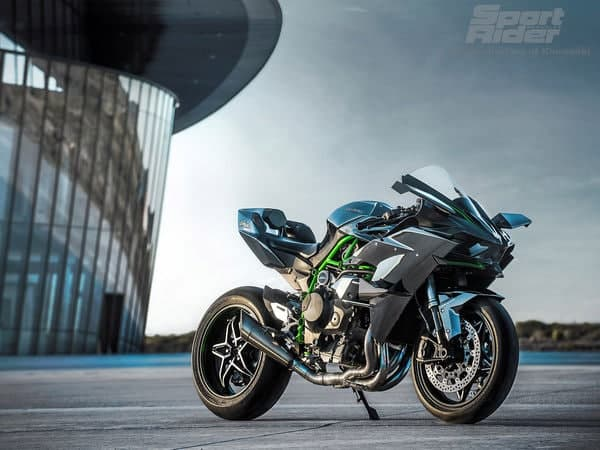
\includegraphics[width=1\linewidth]{images/h2}
			\caption{lhs}
			\label{fig:h1}
		\end{minipage}
		\hspace{0.5cm}
		\begin{minipage}{0.5\linewidth}
			\centering
			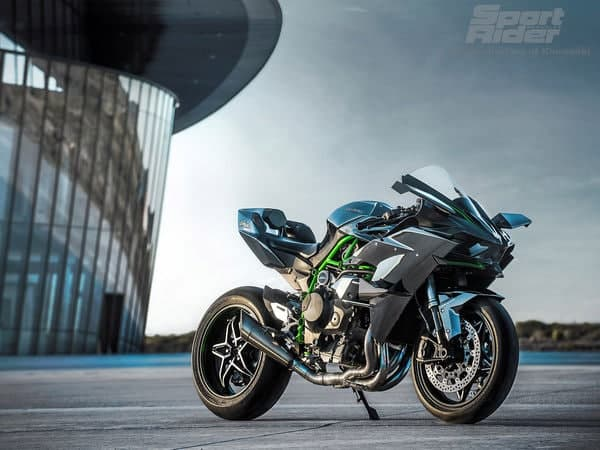
\includegraphics[width=1\linewidth]{images/h2}
			\caption{rhs}
			\label{fig:h3}	
		\end{minipage}		
	\end{figure}
	=======================================	
						%%%%%%%%%%%%%%%%%%%%%%%%%%%%%%%%%%%%%%%%%%%%%%%%%%%%%%%%%%%%%%%%%%%%%%%%%
						
	%% Minipage for placing both tables and subfigures in a single set %%
	\begin{figure}[H]
		\begin{minipage}[b]{0.2\textwidth}
			\centering \fontsize{10}{15}	 
			\captionof{table}{Dimensions of MG-959}
			\begin{tabular}{cc}
				\hline 
				Side & Length (mm) \\ 
				\hline
				A & 43.5 \\ 
				B & 40.2 \\ 
				C & 38 \\  
				D & 20.1 \\
				E & 55 \\
				F & 27 \\
				\hline
			\end{tabular}
			\label{Table 1}	
		\end{minipage}\hspace{2cm}
		\begin{minipage}[b]{0.8\textwidth}
			\begin{subfigure}{0.8\linewidth}
				\centering
				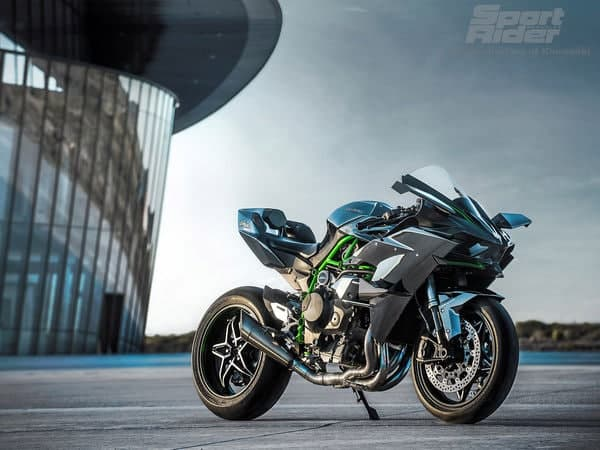
\includegraphics[width=0.6\linewidth]{"images/h2.jpg"}
				\caption{image 6}
				\label{fig:7}
			\end{subfigure}
			\\
			\begin{subfigure}{0.8\linewidth}
				\centering
				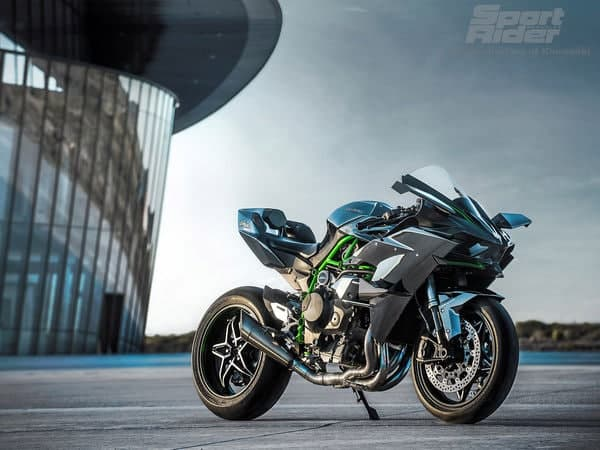
\includegraphics[width=0.6\linewidth]{"images/h2.jpg"}
				\caption{image 7}
				\label{fig:8}
			\end{subfigure} 		 	 		
		\end{minipage}
		\caption{MG-959 Digital Servo technical details}
	\end{figure}
	=======================================	
						%%%%%%%%%%%%%%%%%%%%%%%%%%%%%%%%%%%%%%%%%%%%%%%%%%%%%%%%%%%%%%%%%%%%%%%%%
	
\end{document}